\begin{figure}
  \begin{subfigure}{.5\textwidth}
    \centering
    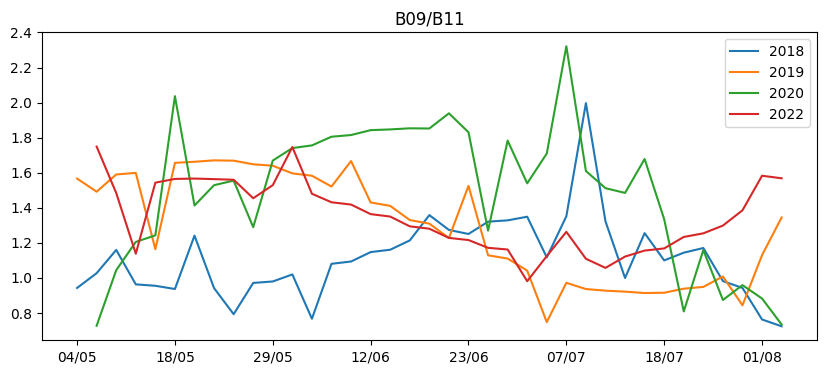
\includegraphics[width=1\linewidth]{figures/curvas_combs/0.png}
    \caption{}
  \end{subfigure}
  \begin{subfigure}{.5\textwidth}
    \centering
    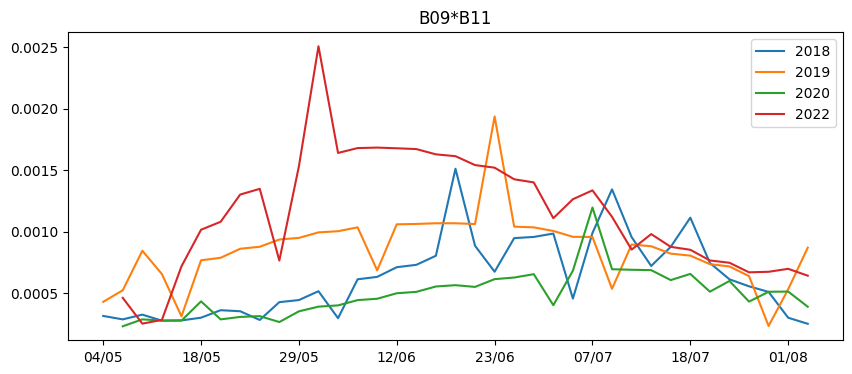
\includegraphics[width=1\linewidth]{figures/curvas_combs/1.png}
    \caption{}
  \end{subfigure}
    \caption{Progresos de las reflectancias de las combinaciones de bandas estudiadas}
    \label{fig:curvas_combs}
\end{figure}

\begin{figure}
  \begin{subfigure}{.5\textwidth}
    \centering
    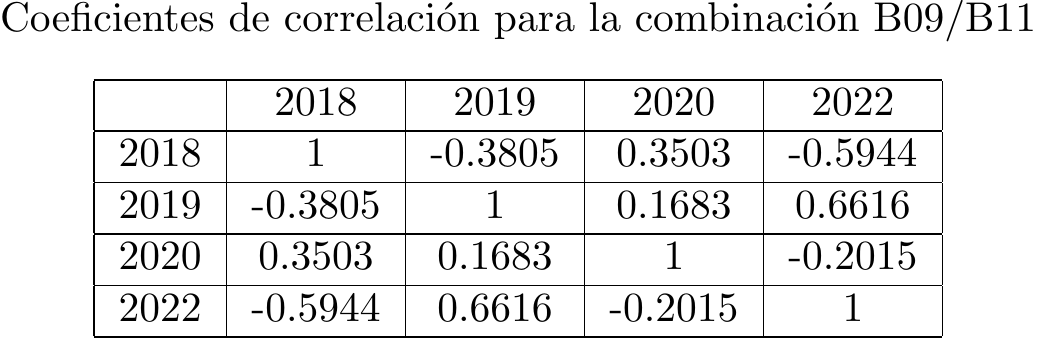
\includegraphics[width=1\linewidth]{figures/curvas_combs/tabla_0.png}
    \caption{}
  \end{subfigure}
  \begin{subfigure}{.5\textwidth}
    \centering
    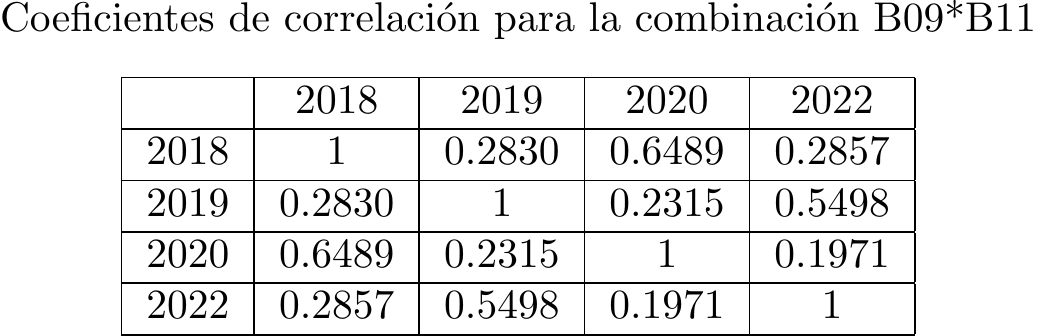
\includegraphics[width=1\linewidth]{figures/curvas_combs/tabla_1.png}
    \caption{}
  \end{subfigure}
    \caption{Correlaciones de las posibles combinaciones de bandas}
    \label{fig:tablas_combs}
\end{figure}